\documentclass[a4paper]{report}
\usepackage[utf8]{inputenc}
\usepackage[T1]{fontenc}
\usepackage{RJournal}
\usepackage{amsmath,amssymb,array}
\usepackage{booktabs}


% tightlist command for lists without linebreak
\providecommand{\tightlist}{%
  \setlength{\itemsep}{0pt}\setlength{\parskip}{0pt}}

\usepackage{longtable}

% Always define CSL refs as bib entries are contained in separate doc
% Pandoc citation processing
\newlength{\cslhangindent}
\setlength{\cslhangindent}{1.5em}
\newlength{\csllabelwidth}
\setlength{\csllabelwidth}{3em}
\newlength{\cslentryspacingunit} % times entry-spacing
\setlength{\cslentryspacingunit}{\parskip}
% for Pandoc 2.8 to 2.10.1
\newenvironment{cslreferences}%
  {}%
  {\par}
% For Pandoc 2.11+
\newenvironment{CSLReferences}[2] % #1 hanging-ident, #2 entry spacing
 {% don't indent paragraphs
  \setlength{\parindent}{0pt}
  % turn on hanging indent if param 1 is 1
  \ifodd #1
  \let\oldpar\par
  \def\par{\hangindent=\cslhangindent\oldpar}
  \fi
  % set entry spacing
  \setlength{\parskip}{#2\cslentryspacingunit}
 }%
 {}
\usepackage{calc}
\newcommand{\CSLBlock}[1]{#1\hfill\break}
\newcommand{\CSLLeftMargin}[1]{\parbox[t]{\csllabelwidth}{#1}}
\newcommand{\CSLRightInline}[1]{\parbox[t]{\linewidth - \csllabelwidth}{#1}\break}
\newcommand{\CSLIndent}[1]{\hspace{\cslhangindent}#1}


\usepackage{amsmath,amssymb,amsthm,array}
\usepackage{booktabs,float,xcolor}
\usepackage[shortlabels]{enumitem}
\newcommand{\tr}{\textcolor{blue}}
\newcommand{\la}{\lambda}
\newcommand{\del}{\delta}
\newcommand{\Ga}{\Gamma}
\newcommand{\La}{\Lambda}
\newcommand{\lra}{\longrightarrow}
\newcommand{\pr}{\prime}
\newcommand{\eps}{\epsilon}
\newcommand{\ga}{\gamma}
\newcommand{\si}{\sigma}
\newcommand{\beq}{\begin{eqnarray}}
\newcommand{\eeq}{\end{eqnarray}}
\newcommand{\bcen}{\begin{center}}
\newcommand{\ecen}{\end{center}}
\newcommand{\ff}{\infty}
\newcommand{\De}{\Delta}
\newcommand{\tB}{\tilde{B}}
\newcommand{\al}{\alpha}
\newcommand{\be}{\beta}
\newcommand{\m}{\omega}
\newcommand{\M}{\Omega}
\newcommand{\sdef}{\stackrel{\mathrm{def}}{=}}
\newcommand{\ka}{\kappa}
\newcommand{\downone}{\vspace{.11in}}
\newcommand{\bth}{\mbox{\boldmath$\theta$}}
\newcommand{\bfG}{\mbox{\boldmath$G$}}
\newcommand{\bfg}{\mbox{\boldmath$g$}}
\newcommand{\bfh}{\mbox{\boldmath$h$}}
\newcommand{\bfD}{\mbox{\boldmath$D$}}
\newcommand{\bfC}{\mbox{\boldmath$C$}}
\newcommand{\bn}{\mbox{\boldmath$n$}}
\newcommand{\bal}{\mbox{\boldmath$\al$}}
\newcommand{\bi}{\mbox{\boldmath$i$}}
\newcommand{\bm}{\mbox{\boldmath$m$}}
\newcommand{\bj}{\mbox{\boldmath$j$}}
\newcommand{\bone}{\mbox{\boldmath$1$}}
\newcommand{\bp}{\mbox{\boldmath$p$}}
\newcommand{\bfy}{\mbox{\boldmath$y$}}
\newcommand{\bx}{\mbox{\boldmath$x$}}
\newcommand{\bz}{\mbox{\boldmath$z$}}
\newcommand{\NN}{{\mathbb N}}
\newcommand{\RR}{{\mathbb R}}
\newcommand{\bzero}{\mbox{\boldmath$0$}}
\newcommand{\calS}{\mathcal{S}}
\newcommand{\calI}{\mathcal{I}}
\newcommand{\calC}{\mathcal{C}}
\newcommand{\calV}{\mathcal{V}}
\newcommand{\caly}{\mathcal{y}}
\newcommand{\calT}{\mathcal{T}}
\newcommand{\calD}{\mathcal{D}}
\newcommand{\calE}{\mathcal{E}}
\newcommand{\bfX}{\mbox{\boldmath$X_n$}}
\newcommand{\tx}{\tilde{x}}

\begin{document}


%% do not edit, for illustration only
\sectionhead{Contributed research article}
\volume{17}
\volnumber{2}
\year{2025}
\month{June}
\setcounter{page}{1}

\begin{article}
  % !TeX root = RJwrapper.tex
\title{Partitioned Local Depth (PaLD) Community Analyses in R}

\author{by Lucy D'Agostino McGowan, Katherine Moore, and Kenneth S. Berenhaut}

\maketitle

\begin{abstract}%
Partitioned Local Depth (PaLD) is a framework for holistic consideration of community structure for distance-based data. This paper describes an R package, pald, for calculating Partitioned Local Depth (PaLD) probabilities, implementing community analyses, determining community clusters, and creating data visualizations to display community structure. We present essentials of the PaLD approach, describe how to use the pald package, walk through several examples, and discuss the method in relation to commonly used techniques.
\end{abstract}

\hypertarget{introduction}{%
\subsection{Introduction}\label{introduction}}

Partitioned Local Depth (PaLD) is a framework for holistic
consideration of community structure for distance-based data. Leveraging
a socially inspired perspective, the approach provides network-based
community information which is founded on new measures of local depth
and pairwise cohesion (partitioned local depth). The method does not
require distributional assumptions, optimization criteria, nor
extraneous inputs. A complete description of the perspective, together
with a discussion of the underlying social motivation, theoretical
results, and applications to additional data sets is provided in \citet{berenhaut2022social}. A brief technical description is included below, directly following the introduction.

As suggested in \citet{berenhaut2022social}, a main goal of PaLD is to ``transform input dissimilarity comparisons into output pairwise relationship strengths (or cohesion) and resulting weighted networks''. This is intended to provide within- and between-community structural information which goes beyond simple cluster labeling. Building on existing approaches to (global) depth, local depth expresses features of centrality via an interpretable probability which is free of parameters and robust to outliers. Partitioning the probabilities which define local depth, we then obtain a measure of cohesion between pairs of individuals. Both local depth and cohesion reflect aspects of relative position (rather than absolute distance) and provide a straightforward
way to account for varying density across the space. As shown in \citet{berenhaut2022social}, provided that two sets are separated (in the sense that the minimum between-set distance is greater than the maximum within-set distance), cohesion is invariant under the contraction and dilation of the distances within each set. This property may be particularly valuable when one has reason to believe that there is heterogeneity in density across the space.

As cohesion captures a sense of the relationship strength between points, we can then analyze and visualize the resulting community structure via a network whose edges are weighted by (mutual) cohesion. The underlying social framework motivates a straightforward yet elegant threshold for distinguishing between strongly and weakly cohesive pairs.

Networks obtained from
cohesion can be displayed using a force-directed graph drawing algorithm; here we will graphically emphasize
the strong ties (colored by connected component). We refer to the
connected components of the network of strong ties as community
``clusters''. Note that to qualify as a cluster in this definition, one
may not have any strong ties with those outside the cluster, and thus
the existence of disjoint groups is a strong signal for separation.
Here, clusters are identified without additional user inputs nor
optimization criteria. If one wishes to further break the community
graph into groups, one may consider using community detection methods
(such as spectral clustering or the Louvain algorithm), as available,
say, in the \CRANpkg{igraph} package. The collection of strong ties may be used in place of
(weighted) \(k\)-nearest neighbors in settings such as classification and
smoothing. Overall, the structural information obtained from local
depth, cohesion and community graphs can provide a holistic perspective
to the data which does not require the use of distributional
assumptions, optimization criteria nor additional user inputs.

It is important to emphasize at the outset that community analyses go beyond simple cluster labeling to address intra- and inter-cluster structure, and can supplement results from other methods for clustering, embedding, data depth, nearest neighbors, etc. In addition, the method does not require distributional assumptions, optimization criteria, nor extraneous inputs. Theoretical considerations (see \citet{berenhaut2022social}) and examples point to distinctive properties that assist in considerations of complex data, in particular with respect to varying density and high dimensions. See the section Cultural and Psychological distance analysis, below, for some discussion in the context of density-based methods.

After a brief introduction to the partitioned
local depth approach (including a concrete and instructive example), below, we present a new package, \CRANpkg{pald}, for calculating partitioned local depths, implementing community analyses, and
creating data visualizations to display community structure. This paper describes how to use the package, walks through several examples, and contrasts the method results with commonly used techniques. Together, these
demonstrate both the novelty of the method and utility of the
implementation in the package described.

\hypertarget{the-partitioned-local-depth-approach}{%
\subsection{The partitioned local depth approach}\label{the-partitioned-local-depth-approach}}

The PaLD methodology as introduced in \citet{berenhaut2022social} offers a parameter-free approach to analyzing community structure in distance-based data. First, consider a ground set \(\mathcal{S}\) equipped with a meaningful measure of pairwise distance (or dissimilarity), \(d:\mathcal{S}\times S\rightarrow \mathbb{R}\cup \infty\). We require only that \(d\) satisfies the requirements that for all \(x,y\in S\) with \(y\neq x\),

\begin{eqnarray}
d(x,x) \leq d(y,x) \mbox{~~~~and~~~~} d(x,x)< d(x,y).
\label{theonereq}
\end{eqnarray}
\noindent Note that \(d\) need not necessarily be symmetric nor positive (see (i) below).

We begin with a concept formalizing locality to a pair. For any pair \((x, y)\in \mathcal{S}\times \mathcal{S}\), the \emph{local focus}, \(U_{x,y}\) (illustrated in Figure \ref{fig:paldmethod} for two-dimensional Euclidean data) is defined via

\begin{eqnarray}
U_{x,y} \stackrel{\text{def}}{=} \{ z \in S \mid d(z,x) \leq d(y,x) \text{ or } d(z,y) \leq d(x,y) \}. \label{localfocusdefn}
\end{eqnarray}

\noindent The set \(U_{x,y}\) is comprised of elements that are ``locally'' relevant to the pair \((x,y)\). Eq. (\ref{theonereq}) guarantees that both \(x\) and \(y\) are elements of \(U_{x,y}\). For discussion from a social perspective, wherein the data are embedded in a latent social space, see Social Framework in \citet{berenhaut2022social}. Recall that in (\ref{localfocusdefn}), the distance \(d\) need not be symmetric; leveraging the social perspective, we are interested in the direct closeness of \(z\) \emph{to} \(x\) and \(y\), not the reverse (see also (iv), below).

\begin{figure}[H]
    \centering
\includegraphics[width=.6\linewidth,trim={2cm 1.2cm 2cm 1cm},clip]{pald-1}

\caption{The local focus for two points, $x$ and $y$, where $\mathcal{S}$ is a subset of $\mathbb{R}^2$, under Euclidean distance (reproduced with permission from \citet{berenhaut2024generalized}). The points in red are outside the focus, $U_{x,y}$. Those in green (and $z$ in blue) are in the focus and closer to $x$, while those in gray are closer to $y$.}\label{fig:paldmethod}
\end{figure}

Now, suppose that \(x\) is fixed, and select \(Y\) and \(Z\) uniformly at random from \(\mathcal{S}\setminus \{x\}\) and \(U_{x,Y}\), respectively. The \emph{local depth} of \(x\), \(\ell_{\mathcal{S}}(x)\), is defined as the probability that \(Z\) is closer to \(x\) than it is to \(Y\) (with a coin flip in the case \(Z\) is equidistant), i.e.

\begin{eqnarray}
\ell_{\mathcal{S}}(x)\stackrel{\mathrm{def}}{=}P(d(Z,x) < d(Z,Y)) \label{localdepthdefn}.
\end{eqnarray}

\noindent The local depth of \(x\) can be thought of as a measure of the extent to which \(x\) is (relatively) surrounded by other elements of \(\mathcal{S}\) (under \(d\)).

Finally, the \emph{cohesion}, \(C_{x,w}\), of \(w\) to \(x\), for a given \(w\in \mathcal{S}\), is obtained through a partitioning of the probability defining local depth in (\ref{localdepthdefn}). In particular,

\begin{eqnarray}
C_{x,w} \stackrel{\mathrm{def}}{=}P(Z=w \mbox{ and } d(Z,x) < d(Z,Y))
\label{cohesdefn}.
\end{eqnarray}

\noindent The cohesion of \(w\) to \(x\) can be viewed as the contribution of \(w\) to the local depth of \(x\). Eq. (\ref{theonereq}) guarantees that when \(Z=x\), \(d(Z,x) < d(Z,Y)\). For some theoretical properties of cohesion, see \citet{berenhaut2022social}. Note that the sum of all cohesions is conserved at \(n/2\), where \(n\stackrel{\mathrm{def}}{=}|\mathcal{S}|\); we thus have a constant mean local depth of \(0.5\) (independent of \(n\)).

A universal threshold for strong cohesion (see \citet{berenhaut2022social}) is defined via

\begin{eqnarray}
T \stackrel{\mathrm{def}}{=}P(Z=W \text{ and } d(Z,X)<d(Z,Y)),
\label{Tsd0}
\end{eqnarray}

\noindent where \(X\), \(Y\), \(Z\), and \(W\) are selected uniformly at random from \(\mathcal{S}\), \(\mathcal{S}\setminus X\), \(U_{X,Y}\), and \(U_{X,Y}\), respectively. The threshold, \(T\), can be conveniently calculated as one half the average of the diagonal of the matrix of pairwise cohesion values (see \citet{berenhaut2022social} for details), i.e.
\begin{equation}
T = \frac{1}{2} \left( \frac{1}{n} \sum_{x\in \mathcal{S}} C_{x,x} \right).
\label{Tsd}
\end{equation}
A strong relationship connection between \(x\) and \(w\) is then established when:
\begin{equation}
\min \{ C_{x,w}, C_{w,x} \} \geq T.
\label{Tsd2}
\end{equation}

For further details on PaLD, including theoretical results, discussion of the underlying social perspective and applications, see \citet{berenhaut2022social} (see also \citet{berenhaut2022SIAM}).

Before moving on to a simple concrete example, we provide a few remarks, for the interested reader, on the concepts introduced above.

\begin{enumerate}[(i)]
\item (Distances and dissimilarities) For the purposes of the package, we require only the inequalities in (\ref{theonereq}). This implies the convenient form of the threshold in (\ref{Tsd2}), see \cite{berenhaut2022social}, and is crucial to the underlying social perspective of conflict. For a more general mathematical PaLD framework, wherein the concepts of locality and support are further refined see \cite{berenhaut2024generalized}. As the definitions in (\ref{localfocusdefn}), (\ref{localdepthdefn}) and (\ref{cohesdefn}) only depend on triplet distance comparisons, local depth and cohesion are invariant under monotone transformations of distance, and negative distances are fine. If meaningful in context, distances need not be symmetric and self-distances, $d(x,x)$, may vary over $x$ (subject to the constraint in (\ref{theonereq})). The triangle inequality may be violated to some extent, mirroring ideas of strong triadic closure (\cite{granovetter1973strength}).

\item (Local foci) The concept of local foci in (\ref{localfocusdefn}) is crucial to all that follows. It allows for consideration of the data at varying scales without the need for localizing parameters. The selection of $Z$ in (\ref{localdepthdefn}) and (\ref{cohesdefn}) reflects the larger presence of individuals in smaller foci (see \cite{feld1981focused} for discussion is social settings). The results in \cite{berenhaut2022social} regarding limiting irrelevance of density and separation under increasing concentration are driven by local comparisons. Self-cohesions (i.e., diagonal elements of $C$) are not necessarily equal. This is driven by the fact that by (\ref{cohesdefn}),
\begin{eqnarray}
C_{x,x}=\frac{1}{n-1} \sum_{y\neq x} \frac{1}{|{U_{x,y}}|},
\end{eqnarray}
\noindent and $C_{x,x}$ is dependent on local density around $x$.

\item (Non-monotonicity of the size of local foci) As distance away from an element, $x$, increases, monotonicity in volume of local foci is not necessary. In particular, consider the one-dimensional set $\mathcal{S}=\{B,x,A,C,D\}$, with $B=5$, $x=11$, $A=16$, $C=18$, $D=19$. Under Euclidean distance, $d(x,A)=5<6=d(x,B)$ but $|U_{x,A}|=|\{x,A,C,D\}|=4$ and $|U_{x,B}|=|\{x,B,A\}|=3$. This further emphasizes the capturing of local density, an important feature of PaLD.

\item (Assymmetry) Note that the definitions in (\ref{localfocusdefn}), (\ref{localdepthdefn}) and (\ref{cohesdefn}) are stated to allow for asymmetric distances, as may occur for instance when considering distances on graphs. Note that even symmetric distances can easily lead to asymmetric cohesion. This is the case even for the simple one-dimensional data considered in Example 1. In considering strong relationships based on cohesion, though, symmetrization is employed in (\ref{Tsd2}).

\item (The use of weighted networks) In what follows, we will at times have occasion to consider a network with node set $\mathcal{S}$ and pairwise edges weighted via the respective values of cohesion. When viewed as a weighted (connectivity) network in this sense,

\begin{enumerate}
\item the weighted nodal degrees are the values of local depth, addressing considerations of (local) data depth,
\item the network may be embedded in low-dimensional Euclidean space via standard network embedding techniques, providing visualization of the data that adapts to relative density,
\item the isolated nodes of either the original network or that restricted to strong ties can provide information regarding outliers,
\item the connected components of the network restricted to strong ties (i.e. those with weights above the threshold in (\ref{Tsd})) can be taken as ``clusters" in the classical sense,
\item weighted or unweighted network neighbors may be used in place of $k$-nearest neighbors in settings such as classification and
smoothing, and
\item some network analyses can be informative regarding data structure.
\end{enumerate}

\noindent Ideas of distance on networks can be complex, though, and this is particularly so for general weighted networks (e.g.  correlation or social networks). As is the case here, edge weights may reflect intensity of connection as opposed to simple pairwise distance, and it is important to exercise caution when applying naïve functions intended for unweighted networks (or simple distance-based weighted networks) in \CRANpkg{igraph} and other software.

\item (Matrix methods) For convenience, we use the \CRANpkg{igraph} package to analyze weighted networks, where appropriate.
Matrix-based methods are also possible. For instance, we employ  \texttt{igraph::components} to obtain community clusters from networks, but alternatively one could use blocks extraction directly from the cohesion matrix using packages such as \CRANpkg{lintools}.

\item (Density-based methods and localized approaches) Complimentary density-based methods such as DBSCAN (density-based spatial clustering of applications with noise) and its hierarchical variant HDBSCAN (see for instance \cite{campello2020density}), seek to identify high-density regions as clusters. We discuss these in the context of a concrete example below (see Cultural and Psychological distance analysis). Determination of required parameter values can be challenging. There are also extent methods for considering data depth which probe local structure (see \cite{paindaveine2013depth} and \cite{agostinelli2011local}). These often also require localizing parameters.
In \citet{berenhaut2022social} (see Theorem 2: Limiting Irrelevance of Density), it is shown that local depth and cohesion account for varying density in the sense that, provided subsets are sufficiently separated, the cohesion is maintained, as within-subset distances are contracted or dilated, without the need to search over a parameter space.

\item (Social latent spaces) The definitions in (\ref{localfocusdefn}), (\ref{localdepthdefn}), (\ref{cohesdefn}), and (\ref{Tsd}), are developed from a social perspective. The interested reader can refer to the section \textit{Social Framework} in \cite{berenhaut2022social}. For further discussion see \cite{berenhaut2024generalized} and \cite{berenhaut2022SIAM}.

\end{enumerate}

\noindent {\bf Example 1.} As a concrete example demonstrating the PaLD framework, consider the one-dimensional set \(\mathcal{S}\stackrel{\mathrm{def}}{=}\{1,3,7,8,9,13,17\}\), with pairwise (Euclidean) distances given in the array below.

\begin{verbatim}
    1  3  7 8 9 13 17
1   0  2  6 7 8 12 16
3   2  0  4 5 6 10 14
7   6  4  0 1 2  6 10
8   7  5  1 0 1  5  9
9   8  6  2 1 0  4  8
13 12 10  6 5 4  0  4
17 16 14 10 9 8  4  0
\end{verbatim}

\noindent The local depths (rounded to three decimal places) are

\begin{verbatim}
    1     3     7     8     9    13    17
0.409 0.463 0.588 0.675 0.600 0.471 0.294
\end{verbatim}

\noindent while the pairwise cohesions (in matrix form) are given by

\begin{Verbatim}[commandchars=\\\{\}]
       1     3     7     8     9    13    17
1  0.210 \tr{0.127} 0.036 0.024 0.012 0.000 0.000
3  \tr{0.137} 0.220 0.048 0.036 0.024 0.000 0.000
7  0.048 0.048 0.220 \tr{0.137} \tr{0.109} 0.028 0.000
8  0.024 0.052 \tr{0.163} 0.218 \tr{0.163} 0.056 0.000
9  0.024 0.024 \tr{0.109} \tr{0.137} 0.220 0.063 0.024
13 0.000 0.000 0.012 0.036 0.103 0.188 \tr{0.133}
17 0.000 0.000 0.000 0.000 0.012 \tr{0.107} 0.175
\end{Verbatim}

\noindent where (non-diagonal) cohesion values above the threshold of
\begin{eqnarray}
0.1036=(1/14) (0.210+0.220+0.220+0.218+0.220+0.188+0.175)
\end{eqnarray}
\noindent are indicated in blue; see (\ref{Tsd2})). The resulting weighted network of pairwise cohesion values is displayed in Figure \ref{fig:figsimple}; here strong ties (with cohesion values above the threshold) are colored according to community clusters (the connected components of the network of strong ties), i.e.~\(\{1,3\}\), \(\{7,8,9\}\) and \(\{13,17\}\).

\begin{figure}[H]
    \centering
\includegraphics[width=3.4in,trim=.2in .4in .2in .4in,clip]{pald-2}

\caption{The community cluster network for the simple one-dimensional data considered in Example 1. Strong ties (with cohesion values above the threshold) are colored according to community clusters (the connected components of the network of strong ties), while weak ties are indicated in grey.}\label{fig:figsimple}
\end{figure}

Note that the cohesion of the element 17 to the element 1 is zero. This reflects the fact that
when an element, \(Y\), other than 1 is selected uniformly at random from \(\mathcal{S}\), and an element \(Z\) is selected uniformly at random from \(U_{x,Y}\), 17 is never, at once, equal to \(Z\) and closer to 1 than it is to the opposing element \(Y\).
In fact, 17 is not an element of \(U_{1,y}\), for \(y\in \{3,7,8\}\). For \(y\in \{9,13,17\}\), \(17\in U_{1,y}\), but in each case, \(d(17,y)<d(17,1)\).
This zero cohesion is reflected in the absence of any edge (grey or colored) from the node for 17 to the node for 1, in Figure \ref{fig:figsimple}. \qed

We now turn to discussion of the \CRANpkg{pald} package.

\hypertarget{pald}{%
\subsection{pald}\label{pald}}

The main functions in the \CRANpkg{pald} package can be split into 3 categories:

\begin{enumerate}
\def\labelenumi{\arabic{enumi}.}
\tightlist
\item
  A function for computing the matrix of cohesion values, as defined in (\ref{cohesdefn}).
\item
  Functions for extracting useful information from the cohesion matrix, such as local depths, neighbors, community clusters, and graph objects.
\item
  Plotting functions for community graphs.
\end{enumerate}

\noindent In addition, the package provides a number of pertinent example data sets which may be used to demonstrate community analysis, including a synthetic data set of two-dimensional points created by \citet{gionis1clustering} to demonstrate aggregation, clustering data generated from the scikit-learn Python package \citep{pedregosa2011scikit}, data describing cognate relationships between words across 87 Indo-European languages \citep{dyen92}, data compiled by \citet{tissue} of tissue gene expressions, data employing information from the World Values Survey \citep{inglehart2014world} on cultural values regarding family, religion, education, and institutions for several regions \citep{muthukrishna2020beyond}, and three example data sets generated for the \citet{berenhaut2022social} paper.

While it is not a necessity, the \CRANpkg{pald} package is designed to function well with the pipe operator, \texttt{\textbar{}\textgreater{}}, particularly for those who are familiar with tidyverse-based approaches. This functionality will be demonstrated briefly below.

\hypertarget{creating-the-cohesion-matrix}{%
\subsubsection{Creating the cohesion matrix}\label{creating-the-cohesion-matrix}}

For the purposes of the \CRANpkg{pald} package, the sole input for the Partitioned Local Depth (PaLD) computations is a distance matrix or \texttt{dist} object. Recall that the collection of input distances (or dissimilarities) is assumed to satisfy the requirements in (\ref{theonereq}). More generally, the method only requires triplet distance comparisons, as opposed to exact numeric distances (see \citet{berenhaut2022social}).

For demonstration purposes, we first show how one can compute a distance matrix from an input data frame with, say, two variables \texttt{x1} and \texttt{x2}. The input data may be of any dimension; in fact the PaLD framework provides advantages when considering high-dimensional data (see the \textbf{Examples} section as well as \citet{berenhaut2022social}).

\begin{verbatim}
library(pald)
df <- data.frame(
  x1 = c(6, 8, 8, 16, 4, 14),
  x2 = c(5, 4, 10, 8, 4, 10)
)
rownames(df) <- c("A", "B", "C", "D", "E", "F")
\end{verbatim}

The \texttt{dist} function returns a (default Euclidean) pairwise distance matrix for an input data frame, as demonstrated below. If the data are already provided as a distance matrix (or \texttt{dist} object), the user can skip to the next step. Note that the distance matrix needed for the subsequent functions does not need to be a \texttt{dist} object and \emph{need not} be symmetric.

\begin{verbatim}
d <- dist(df)
\end{verbatim}

The function above creates a \texttt{dist} object. If converted to a matrix, this will be an \(n\times n\) distance matrix, where \(n\) corresponds to the number of observations in the original data frame (in this example \(n = 6\)).

This \texttt{dist} object, or a distance matrix, can then be passed to the \texttt{cohesion\_matrix} function in order to calculate pairwise cohesion values.

\begin{verbatim}
cohesion_matrix(d)
\end{verbatim}

\begin{verbatim}
#>            A          B          C         D          E         F
#> A 0.25000000 0.18333333 0.06666667 0.0000000 0.18333333 0.0000000
#> B 0.14000000 0.24000000 0.05000000 0.0000000 0.10666667 0.0000000
#> C 0.07333333 0.07333333 0.20333333 0.0000000 0.03333333 0.0800000
#> D 0.00000000 0.00000000 0.00000000 0.2333333 0.00000000 0.1333333
#> E 0.14000000 0.10666667 0.03333333 0.0000000 0.24000000 0.0000000
#> F 0.00000000 0.00000000 0.05000000 0.1400000 0.00000000 0.2400000
#> attr(,"class")
#> [1] "cohesion_matrix" "matrix"          "array"
\end{verbatim}

Equivalently, the user can use the native pipe \texttt{\textbar{}\textgreater{}} as follows.

\begin{verbatim}
df |>
  dist() |>
  cohesion_matrix()
\end{verbatim}

\begin{verbatim}
#>            A          B          C         D          E         F
#> A 0.25000000 0.18333333 0.06666667 0.0000000 0.18333333 0.0000000
#> B 0.14000000 0.24000000 0.05000000 0.0000000 0.10666667 0.0000000
#> C 0.07333333 0.07333333 0.20333333 0.0000000 0.03333333 0.0800000
#> D 0.00000000 0.00000000 0.00000000 0.2333333 0.00000000 0.1333333
#> E 0.14000000 0.10666667 0.03333333 0.0000000 0.24000000 0.0000000
#> F 0.00000000 0.00000000 0.05000000 0.1400000 0.00000000 0.2400000
#> attr(,"class")
#> [1] "cohesion_matrix" "matrix"          "array"
\end{verbatim}

The \emph{cohesion matrix} output by the \texttt{cohesion\_matrix} function is the main input for the majority of the remaining functions.

\hypertarget{functions-for-extracting-information-from-the-cohesion-matrix}{%
\subsubsection{Functions for extracting information from the cohesion matrix}\label{functions-for-extracting-information-from-the-cohesion-matrix}}

From the \emph{cohesion matrix}, a variety of useful quantities can be computed. Below, we create a cohesion matrix using the functions described in the previous section.

\begin{verbatim}
df |>
  dist() |>
  cohesion_matrix() -> cohesion
\end{verbatim}

The \texttt{local\_depths} function calculates the \emph{depth} of each point, as defined in (\ref{localdepthdefn}), outputting a vector of local depth probabilities.

\begin{verbatim}
local_depths(cohesion)
\end{verbatim}

\begin{verbatim}
#>         A         B         C         D         E         F
#> 0.6833333 0.5366667 0.4633333 0.3666667 0.5200000 0.4300000
\end{verbatim}

\noindent In this case, the (locally) deepest point is \texttt{A}.

The \texttt{strong\_threshold} function will calculate the cohesion threshold for strong ties given in (\ref{Tsd0}), which reflects typical cohesion for local points (see \citet{berenhaut2022social}). Computationally, this is equal to half the average of the diagonal of the cohesion matrix, and is a threshold that may be used to distinguish between strong and weak ties.

\begin{verbatim}
strong_threshold(cohesion)
\end{verbatim}

\begin{verbatim}
#> [1] 0.1172222
\end{verbatim}

\noindent Here, the threshold is a little above \texttt{0.117}.

The function \texttt{cohesion\_strong} will update the cohesion matrix to set all weak ties to zero (via the \texttt{strong\_threshold} function). Reflecting (\ref{Tsd2}), by default, the matrix will also be symmetrized, using the entry-wise (parallel) minimum of the cohesion matrix and its transpose.

\begin{verbatim}
cohesion_strong(cohesion)
\end{verbatim}

\begin{verbatim}
#>      A    B         C         D    E         F
#> A 0.25 0.14 0.0000000 0.0000000 0.14 0.0000000
#> B 0.14 0.24 0.0000000 0.0000000 0.00 0.0000000
#> C 0.00 0.00 0.2033333 0.0000000 0.00 0.0000000
#> D 0.00 0.00 0.0000000 0.2333333 0.00 0.1333333
#> E 0.14 0.00 0.0000000 0.0000000 0.24 0.0000000
#> F 0.00 0.00 0.0000000 0.1333333 0.00 0.2400000
#> attr(,"class")
#> [1] "cohesion_matrix" "matrix"          "array"
\end{verbatim}

The \texttt{community\_graphs} function takes the cohesion matrix and creates \CRANpkg{igraph} objects, graphs that describe the (symmetrized) relationship structure between points. This function will output a list of three objects:

\begin{itemize}
\tightlist
\item
  \texttt{G}: the weighted (community) graph whose edge weights are mutual cohesion
\item
  \texttt{G\_strong}: the weighted (community) graph consisting of edges for which mutual (symmetrized) cohesion (i.e.~the minimum of the two directed cohesion values for any given pair) is greater than the threshold for strong ties
\item
  \texttt{layout}: the graph layout. By default this is provided by the Fruchterman Reingold (FR) force-directed graph drawing algorithm for the graph \texttt{G}, as implemented in the \CRANpkg{igraph} package.
\end{itemize}

\begin{verbatim}
graphs <- community_graphs(cohesion)
graphs[["G_strong"]]
\end{verbatim}

\begin{verbatim}
#> IGRAPH c4d81a7 UNW- 6 3 --
#> + attr: name (v/c), weight (e/n)
#> + edges from c4d81a7 (vertex names):
#> [1] A--B A--E D--F
\end{verbatim}

Here we see that there are three connected components, ties \texttt{A-B} and \texttt{A-E} form the first community cluster, and the tie \texttt{D-F} which forms another.

The \texttt{any\_isolated()} function will check whether there are any isolated points (according to cohesion).

\begin{verbatim}
any_isolated(cohesion)
\end{verbatim}

\noindent Here, there are no isolated points, i.e.~points having zero cohesion with all other points in the data (an extreme form of outlier).

The ``community clusters'' identified by PaLD are the connected components of the graph of strong ties, \texttt{G\_strong}. To directly calculate these, we can use the \texttt{community\_clusters} function. This will output a data frame with two columns; the first corresponds to the individual (\texttt{point}), as identified by the row name of the original input data frame, \texttt{df}, the second identifies the \texttt{community} that the individual belongs to.

\begin{verbatim}
community_clusters(cohesion)
\end{verbatim}

\begin{verbatim}
#>   point community
#> A     A         1
#> B     B         1
#> C     C         2
#> D     D         3
#> E     E         1
#> F     F         3
\end{verbatim}

In this example, three communities are identified with these six points. Points \texttt{A}, \texttt{B}, and \texttt{E} fall into Community 1. Point \texttt{C} is in Community 2 (a community of size 1) and points \texttt{D} and \texttt{F} fall into Community 3.

\hypertarget{plotting-functions}{%
\subsection{Plotting functions}\label{plotting-functions}}

The final category of function is that for data visualization. We can begin by visualizing the points in the data frame \texttt{df} (Figure \ref{fig:fig1}). When visualizing these points, it is important to have the aspect ratio of the x and y axes equal to 1 so as to not distort distances. When using the \CRANpkg{ggplot2} package for this visualization, one can use the command \texttt{coord\_fixed(ratio\ =\ 1)}. If using the \texttt{plot} function included in the base library, one can use the \texttt{asp\ =\ 1} argument.

\begin{verbatim}
library(ggplot2)
ggplot(df, aes(x1, x2)) +
  geom_text(label = rownames(df)) +
  coord_fixed(ratio = 1) +
  xlim(c(4, 16)) +
  ylim(c(4, 16))
\end{verbatim}

\begin{figure}[H]
\centering
\includegraphics[width=4in,trim=0in 0in 0in 0in,clip]{dagostino-mcgowan_files/figure-latex/fig1-1}

\caption{Visualization of the points from the data frame \texttt{df}}\label{fig:fig1}
\end{figure}

We can pass the cohesion matrix to the \texttt{plot\_community\_graphs} function to view the relationship between points (Figure \ref{fig:fig2}). The function will also permit parameters that can be passed to \texttt{plot.igraph} via the \texttt{...} argument.

\begin{verbatim}
plot_community_graphs(cohesion,
                      vertex.label.cex = 2,
                      vertex.label.dist = 0.9)
\end{verbatim}

\begin{figure}[H]
\centering\includegraphics[width=4in,trim=0in .4in 0in .4in,clip]{dagostino-mcgowan_files/figure-latex/fig2-1.pdf}
\caption{\label{fig:fig2}PaLD graph displaying the relationship between the points in data frame \texttt{df}}
\end{figure}

Notice in this plot the force-directed layout does not match that of the original data frame as seen in Figure \ref{fig:fig1}. Since our original data is two-dimensional, it may be reasonable to use the latter as the layout for plotting. Figure \ref{fig:fig3} includes this update as well as others addressing some of the aesthetics, such as employing more readable labels. The \texttt{layout} argument allows the user to pass a matrix to dictate the 2-dimensional layout of the graph. For example, if we wanted the graph to match the visualization displayed in Figure \ref{fig:fig1}, we could pass \texttt{as.matrix(df)} (a matrix of the data frame \texttt{df}) to the \texttt{layout} argument (Figure \ref{fig:fig3}). Here, we increase the vertex size and change the vertex label color, through the argument specifications \texttt{vertex.size\ =\ 100} and \texttt{vertex.label.color\ =\ "white"}. Additionally, to allow axes, we use \texttt{axes\ =\ TRUE}, and to put these back on the original scale we set \texttt{rescale\ =\ FALSE}, resetting the axis limits using \texttt{xlim} and \texttt{ylim}. The \texttt{par(pty\ =\ "s")} function forces the subsequent plot to be square.

\begin{verbatim}
par(pty = "s")

plot_community_graphs(cohesion,
                      layout = as.matrix(df),
                      vertex.size = 100,
                      vertex.label.color = "white",
                      axes = TRUE,
                      rescale = FALSE,
                      asp = 1,
                      xlim = c(4, 16),
                      ylim = c(4, 16))
\end{verbatim}

\begin{figure}[H]
\centering
\includegraphics[width=4.6in,trim=1in .6in 1in .68in,clip]{dagostino-mcgowan_files/figure-latex/fig3-1.pdf}
\caption{\label{fig:fig3}PaLD graph displaying the relationship between the points in data frame \texttt{df}, matching the original layout in Figure \ref{fig:fig1}}
\end{figure}

\hypertarget{examples}{%
\subsection{Examples}\label{examples}}

We will demonstrate the utility of the \CRANpkg{pald} package through several illustrative examples.

\hypertarget{community-analysis-for-tissue-gene-expression-data}{%
\subsubsection{Community analysis for tissue gene expression data}\label{community-analysis-for-tissue-gene-expression-data}}

The first example is from a subset of data from \citet{zilliox2007gene}, \citet{mccall2011gene}, and \citet{mccall2014gene}, obtained from the \textbf{tissuesGeneExpression} bioconductor package \citep{tissue} consisting of 22,215-dimensional gene expression data from 189 tissue samples. A (Euclidean) \texttt{dist} object was created using this data set and is included in the \CRANpkg{pald} package in an object called \texttt{tissue\_dist}.

The \texttt{tissue\_dist} object is a \texttt{dist} object resulting in a distance matrix with 189 rows and 189 columns.

We can create the cohesion matrix using the \texttt{cohesion\_matrix} function.

\begin{verbatim}
tissue_cohesion <- cohesion_matrix(tissue_dist)
\end{verbatim}

We can display relationships between tissue samples, both locally and globally through the \texttt{plot\_community\_graphs} function (Figure \ref{fig:fig4}). For clarity of the display, we show how to remove the labels using \texttt{show\_labels\ =\ FALSE}. We will instead color according to the labels by passing these to the \texttt{vertex.color} argument for the \texttt{plot.igraph} function (via the \texttt{...} argument). Similarly, we can add a legend using the \texttt{legend()} function, as you would for an \CRANpkg{igraph} visualization. Additionally, we use the \texttt{edge\_width\_factor} and \texttt{emph\_strong} arguments to adjust the width of the lines between and within PaLD communities.

\begin{verbatim}
labels <- rownames(tissue_cohesion)
plot_community_graphs(tissue_cohesion,
                      show_labels = FALSE,
                      vertex.size = 4,
                      vertex.color = as.factor(labels),
                      edge_width_factor = 35,
                      emph_strong = 5)
legend("topleft",
       legend = unique(as.factor(labels)),
       pt.bg = unique(as.factor(labels)),
       col = "black",
       pch = 21)
\end{verbatim}

\begin{figure}[H]
\centering
\includegraphics[width=5in,trim=0in 3in 0in 3in,clip]{fig5} \caption{Community cluster network for the tissue data. The line colors indicate the PaLD communities; the point colors indicate the tissue classification.}\label{fig:fig4}
\end{figure}

A summary of community strong ties can be produced via the following code. Note that \texttt{tissue\_graph\_strong} is an \CRANpkg{igraph} object corresponding to the graph displayed in Figure \ref{fig:fig4}, restricted only to strong ties.

\begin{verbatim}
tissue_graphs <- community_graphs(tissue_cohesion)
tissue_graph_strong <- tissue_graphs[["G_strong"]]
E <- igraph::get.edgelist(tissue_graph_strong)
tissue_strong_ties <- data.frame(
  strong_ties = apply(E, 1, paste, collapse = ",")
)
tissue_strong_ties |>
  table() |>
  sort(decreasing = TRUE)
\end{verbatim}

\begin{verbatim}
#> strong_ties
#>           kidney,kidney
#>                     273
#>             colon,colon
#>                     241
#> hippocampus,hippocampus
#>                     191
#>   cerebellum,cerebellum
#>                     186
#>             liver,liver
#>                      85
#> endometrium,endometrium
#>                      81
#>       placenta,placenta
#>                       4
#>      kidney,endometrium
#>                       3
\end{verbatim}

Note that there are only three strong ties between different tissue types (kidney and endometrium) in the community cluster network of 1,064 strong ties total.

\hypertarget{cognate-based-language-families}{%
\subsection{Cognate-based Language Families}\label{cognate-based-language-families}}

This example explores a data set from \citet{dyen92} that summarizes relationships between 87 Indo-European languages from the perspective of cognates, coded using 2,655-dimensional binary vectors. A \texttt{dist} object was created from this data set and is included in the \CRANpkg{pald} package in an object called \texttt{cognate\_dist}.

Here we will demonstrate how one can further apply functions in the \CRANpkg{igraph} package to objects output from the \CRANpkg{pald} package. We can first use the \texttt{cohesion\_matrix} function to calculate the cohesion matrix and the \texttt{community\_graphs} function to create a list with the weighted community graph, the weighted community graph with only strong ties included, and the layout. From this, we can extract the graph with only the strong ties, here called \texttt{cognate\_graph\_strong}.

\begin{verbatim}
cognate_cohesion <- cohesion_matrix(cognate_dist)
cognate_graphs <- community_graphs(cognate_cohesion)

cognate_graph_strong <- cognate_graphs[["G_strong"]]
\end{verbatim}

We can then use the \texttt{neighbors} function from the \CRANpkg{igraph} package to extract the strong neighbors in this graph. For example, we can extract all neighbors for the language ``French'', via the following code.

\begin{verbatim}
french_neighbors <- igraph::neighbors(cognate_graph_strong, "French")
french_neighbors
\end{verbatim}

\begin{verbatim}
#> + 8/87 vertices, named, from 5c6bb3a:
#> [1] Italian
#> [2] Ladin
#> [3] Provencal
#> [4] Walloon
#> [5] French_Creole_C
#> [6] French_Creole_D
#> [7] Spanish
#> [8] Catalan
\end{verbatim}

Similarly, we can sort and print the associated neighborhood weights by subsetting the cohesion matrix.

\begin{verbatim}
cognate_cohesion["French", french_neighbors] |>
  sort(decreasing = TRUE)
\end{verbatim}

\begin{verbatim}
#>         Walloon
#>      0.03258771
#>       Provencal
#>      0.02871174
#> French_Creole_C
#>      0.02406057
#> French_Creole_D
#>      0.02406057
#>           Ladin
#>      0.02094596
#>         Italian
#>      0.01997696
#>         Catalan
#>      0.01859688
#>         Spanish
#>      0.01679733
\end{verbatim}

We can again use the \texttt{plot\_community\_graphs} function to visualize the community clusters (Figure \ref{fig:figlang}). One may note the commonly identifiable language clusters and that, under a slight rotation, some of the underlying geography is mirrored in the plot.

\begin{verbatim}
plot_community_graphs(
  cognate_cohesion,
  edge_width_factor = 30,
  emph_strong = 3,
  vertex.size = 3,
  vertex.label.cex = 0.7,
  vertex.label.dist = 1
)
\end{verbatim}

\begin{figure}[H]
\centering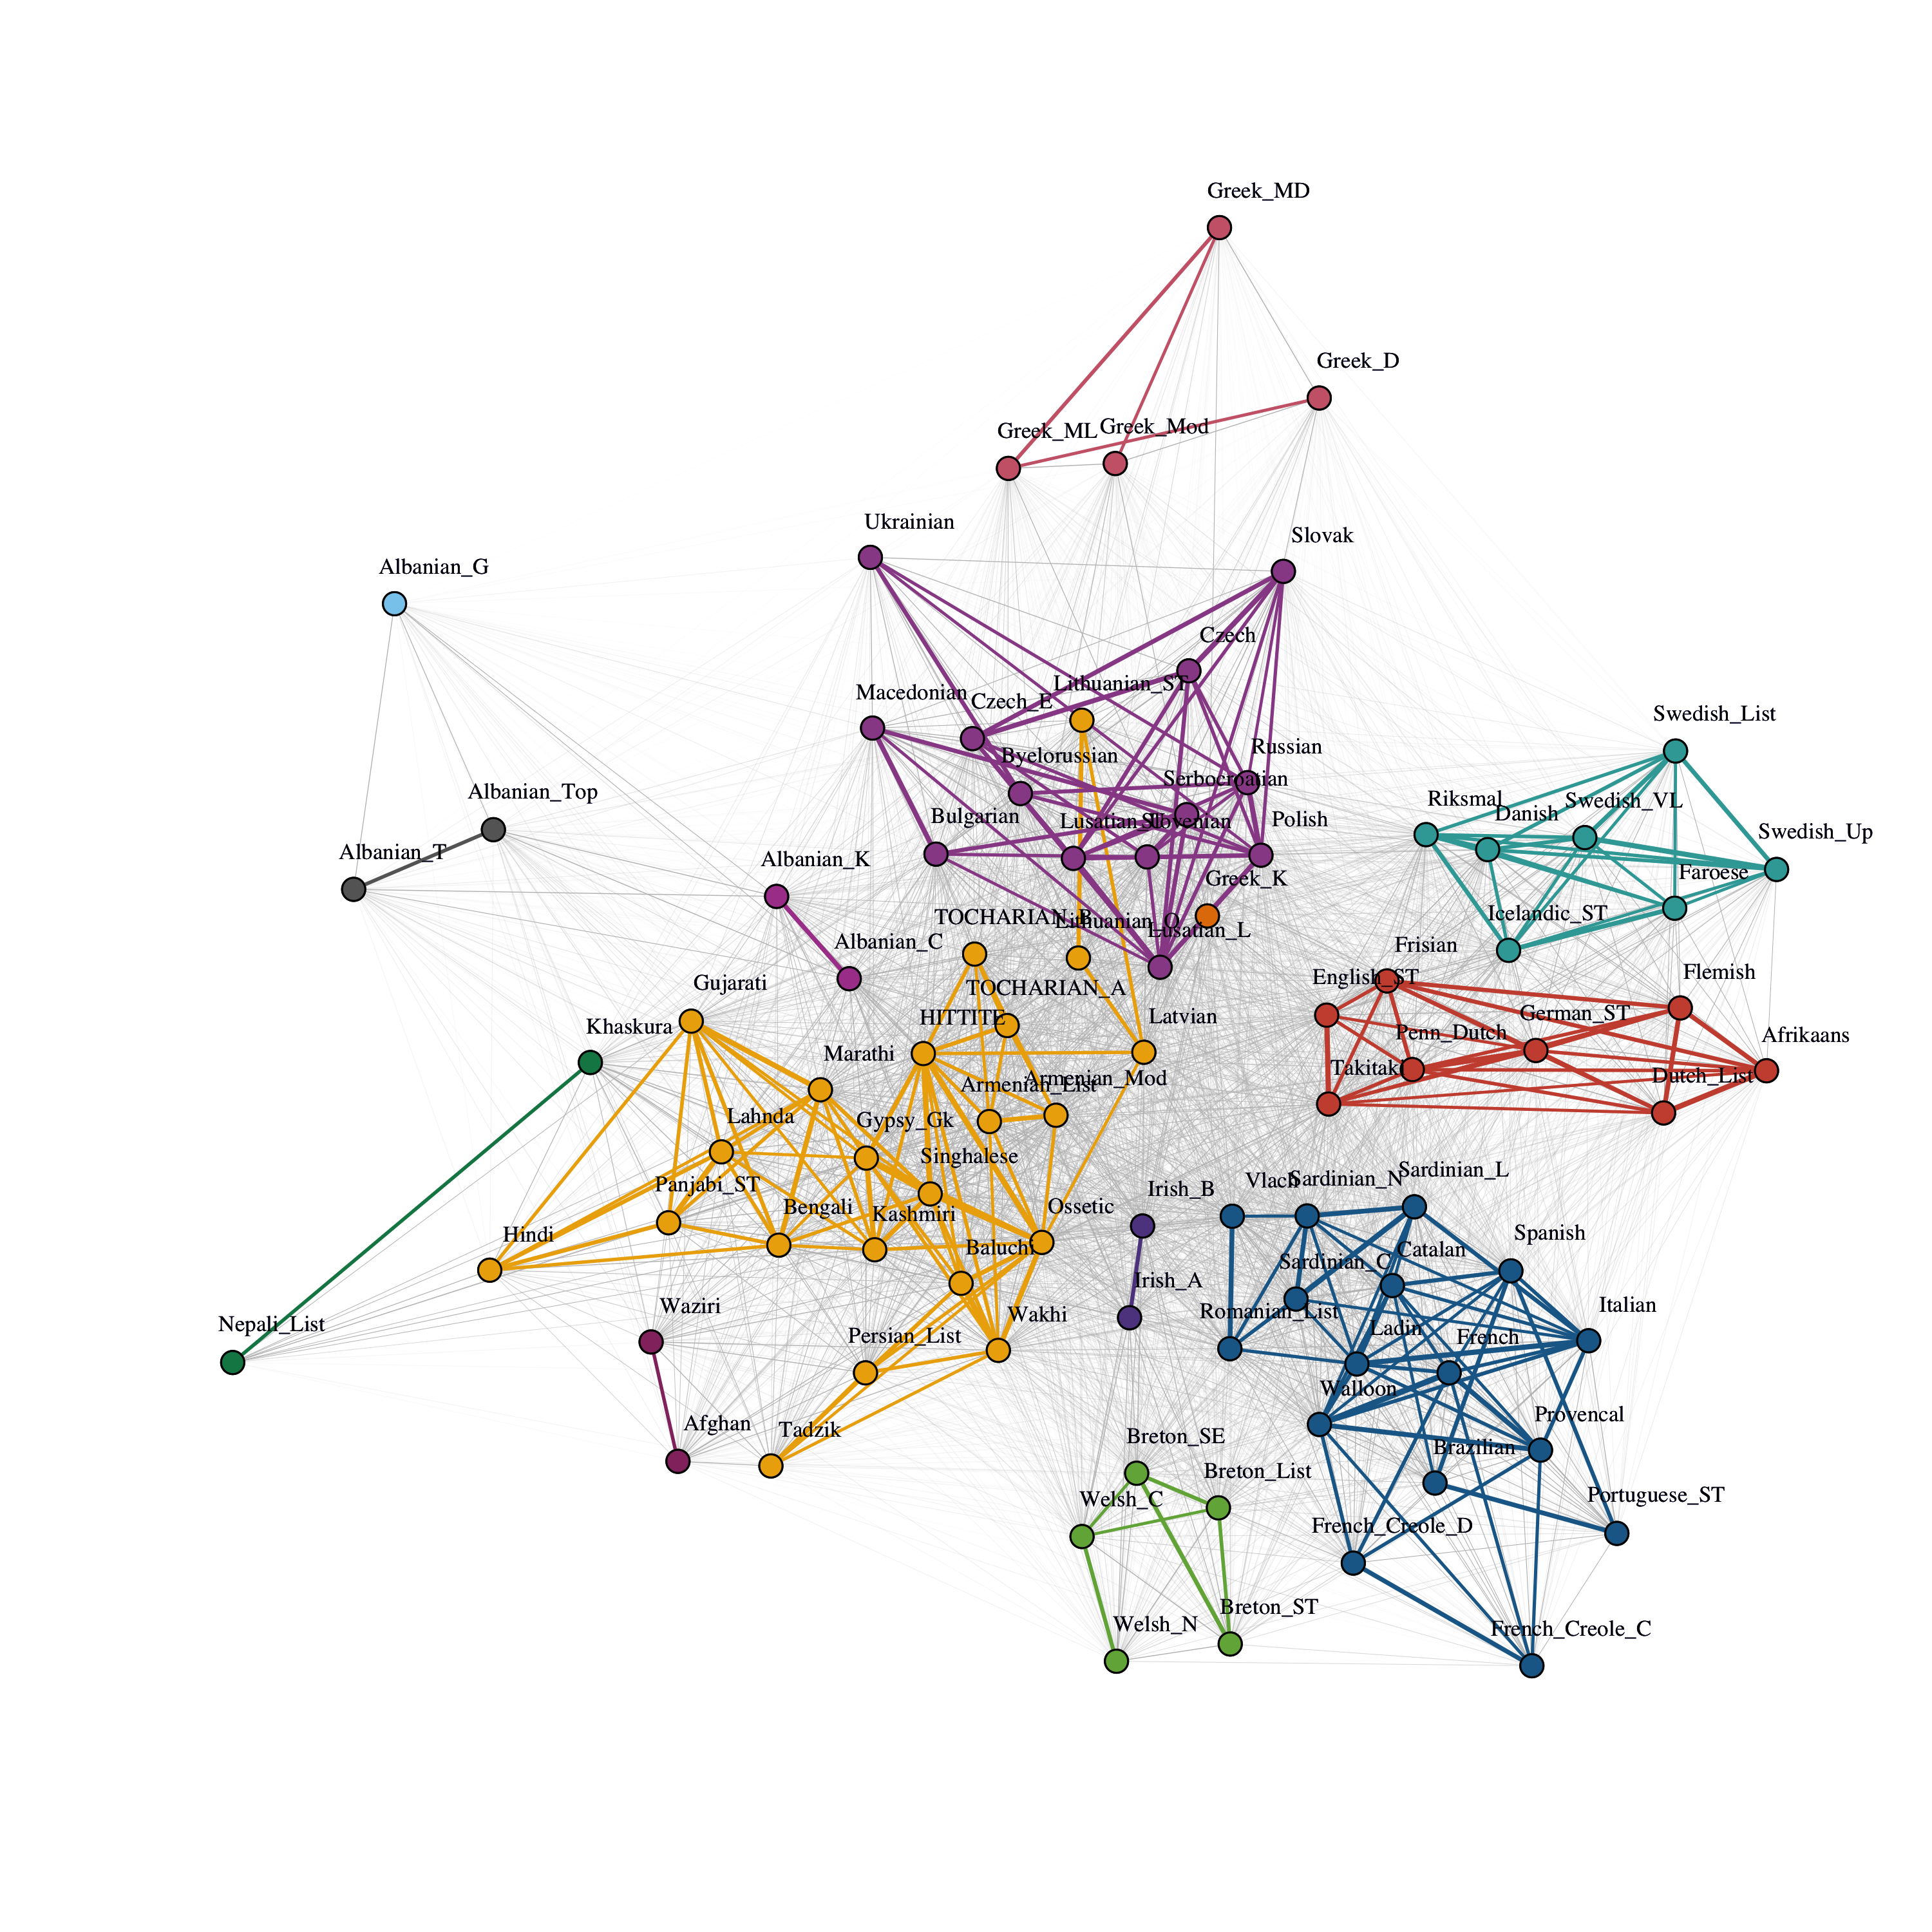
\includegraphics[width=5.6in,trim=1.5in 4in 2.2in 1.95in,clip]{fig6} \caption{Community structure for 87 Indo-European languages, which employs cognate information that was coded via 2,665-dimensional binary vectors. Commonly identifiable language clusters arise along with informative inter- and intra-cluster structure. Several ancient languages are centrally located.}\label{fig:figlang}
\end{figure}

\hypertarget{community-analysis-for-generated-data}{%
\subsubsection{Community analysis for generated data}\label{community-analysis-for-generated-data}}

The \CRANpkg{pald} package includes three randomly generated data frames corresponding to plots from \citet{berenhaut2022social}:

\begin{itemize}
\tightlist
\item
  \texttt{exdata1} is a data set consisting of 8 points used to create Figure 1 in \citet{berenhaut2022social}
\item
  \texttt{exdata2} is a data set consisting of 16 points used to create Figure 2 in \citet{berenhaut2022social}
\item
  \texttt{exdata3} is a data set consisting of 240 points used to create Figure 4D in \citet{berenhaut2022social}
\end{itemize}

Here, we will demonstrate how to use \texttt{exdata3}. These points were generated from bivariate normal distributions with varying means and variances. There are eight ``true'' communities.

We can contrast resulting community clusters obtained via PaLD (i.e.~connected components of the network of strong ties) with clusters as obtained through common cluster analysis techniques. Here we will consider two common clustering methods. The code below calculates the cohesion matrix (\texttt{exdata\_cohesion}) as well as the community clusters obtained via PaLD (\texttt{exdata\_pald}), along with \(k=8\) clusters obtained via \emph{k}-means (\texttt{exdata\_kmeans}) and hierarchical clustering using complete linkage (\texttt{exdata\_hclust}). Recall that there is no need to determine values for extraneous inputs in the case of PaLD (e.g.~the number of clusters, as is necessary to specify for \emph{k}-means and hierarchical clustering).

\begin{verbatim}
exdata_cohesion <- exdata3 |>
  dist() |>
  cohesion_matrix()

exdata_pald <- community_clusters(exdata_cohesion)$community

exdata_kmeans <- kmeans(exdata3, 8)$cluster

exdata_hclust <- exdata3 |>
  dist() |>
  hclust() |>
  cutree(k = 8)
\end{verbatim}

The information is displayed in Figure \ref{fig:fig5}.

\begin{verbatim}
par(mfrow = c(1, 3), pty = "s")
plot(
  exdata3,
  pch = 16,
  col = pald_colors[exdata_pald],
  xlab = "",
  ylab = "",
  main = "PaLD Communities",
  asp = 1
)
plot(
  exdata3,
  pch = 16,
  col = pald_colors[exdata_kmeans],
  xlab = "",
  ylab = "",
  main = "K-Means Clusters (k = 8)",
  asp = 1
)
plot(
  exdata3,
  pch = 16,
  col = pald_colors[exdata_hclust],
  xlab = "",
  ylab = "",
  main = "Hiearchical Clusters (k = 8)",
  asp = 1
)
\end{verbatim}

\begin{figure}[H]
\centering
\includegraphics[width=5in,trim=0in 1in 0in .4in,clip]{dagostino-mcgowan_files/figure-latex/fig5-1.pdf}
\caption{\label{fig:fig5}PaLD, k-means, and hierarchical 8-clustering of randomly generated example data (from \citet{berenhaut2022social}; Figure 4D).}
\end{figure}

Cohesion is particularly useful when considering data with varying local density; see \citet{berenhaut2022social} for further examples, discussion, and theoretical results. Note that the PaLD algorithm is able to detect the eight natural groups within the data (along with inter- and intra-community structure not displayed here) without the use of any additional inputs (e.g., number of clusters) nor optimization criteria. Despite the user input of the ``correct'' number of clusters (i.e., \(k = 8\)) both \emph{k}-means and hierarchical clustering do not provide the desired result.

\hypertarget{cultural-and-psychological-distance-analysis}{%
\subsubsection{Cultural and Psychological distance analysis}\label{cultural-and-psychological-distance-analysis}}

In this example we perform a PaLD analysis for cultural distances obtained in \citet{muthukrishna2020beyond} from two recent waves of the World Values Survey (2005 to 2009 and 2010 to 2014; see \citet{inglehart2014world}). Distances are
computed using the cultural fixation index (CFST), which is a measure built on the framework of fixation indices from population
biology (\citet{bell2009culture,cavalli1994history}). Recall that the foundation of PaLD in within-triplet comparisons allows for the employment of application-dependent and non-Euclidean measures of dissimilarity.
The \texttt{dist} object is
included in the \CRANpkg{pald} package (\texttt{cultures}). We will first create the cohesion matrix using the \texttt{dist} object \texttt{cultures}, and proceed to plot the community graph.

\begin{verbatim}
cultures_cohesion <- cohesion_matrix(cultures)
\end{verbatim}

\begin{verbatim}
plot_community_graphs(
  cultures_cohesion,
  edge_width_factor = 30,
  emph_strong = 3,
  vertex.label.cex = 0.7,
  vertex.size = 3,
  vertex.label.dist = 1
)
\end{verbatim}

\begin{figure}[H]
\centering
\includegraphics[width=5.4in,trim=1in 3in 1in 1in,clip]{fig7} \caption{Community structure for cultural distance data.}\label{fig:figculture}
\end{figure}

In addition to viewing the local and global community structure as seen in Figure \ref{fig:figculture}, the \CRANpkg{pald} package allows for a two-dimensional display of cohesion against distance for the data, via the \texttt{dist\_cohesion\_plot} function, as seen below (Figure \ref{fig:figco}).

\begin{verbatim}
dist_cohesion_plot(cultures, mutual = TRUE)
\end{verbatim}

\begin{figure}[H]
\centering
\includegraphics[width=3.7in,trim=0in .4in 0in .7in,clip]{dagostino-mcgowan_files/figure-latex/figco-1.pdf}
\caption{\label{fig:figco}A plot of cohesion versus distance for the data. The identified communities are colored as in Figure \ref{fig:figculture}.}
\end{figure}

Notice here that the magnitude of the distances within each of the identified communities varies substantially between regions; in fact, the most disparate two regions in the United States (at distance \(\approx\) 0.027) are far closer than the two most similar in India (at distance \(\approx\) 0.043). Despite this, India remains a cohesive whole, and locally disparate regions in the United States such as East South Central and California are not strongly cohesive. For discussion of subtleties in local density (see \citet{berenhaut2022social}. Additionally, currently available techniques require specification of parameters, as seen in the previous section. For further discussion of the cultural distance data in relation to community analysis see \citet{berenhaut2022social}.

Given the inherent variation in density over regions, it is of interest to consider complementary results from density-based methods such as DBSCAN and its variant HDBSCAN. Employing the \CRANpkg{dbscan} package (see \citet{hahsler2019dbscan}), for DBSCAN with parameters \texttt{eps=0.34} and \texttt{minPts=3}, we have a result with five clusters and six regions being classified as noise. Therein, (excluding noise) the Indian region is split into two communities. Similarly, for HDBSCAN, with \texttt{minPts=3}, we have a result with five clusters and eight noise points. Here again (excluding the noise points), India has been split into two communities. The parameter choices used for both methods were determined by maximizing normalized mutual information (NMI; see \citet{ana2003robust}), when comparing with the underlying partition of the regions into Europe, United States, India and China, by regional information), giving values of 0.848 and 0.819, respectively. For comparison, the corresponding NMI value for the result in Figure 9 is 0.933. Further discussion is available in \citet{berenhaut2022social}. It is important to note the required parameter choices for both DBSCAN and HDBSCAN and that results can be somewhat sensitive to changes in these. For instance, for DBSCAN, an increase in the value of \texttt{minPts} from \(3\) to \(5\), and a decrease in \texttt{eps} value from \(0.34\) to \(0.30\) leads to a large number of noise points (25), and a decrease in NMI value from \(0.848\) to \(0.685\). For HDBSCAN an increase in the value of \texttt{minPts} from \(3\) to \(5\) leads to 15 noise points, and a decrease in NMI value from \(0.819\) to \(0.760\), while a decrease in the value of \texttt{minPts} from \(3\) to \(2\) leads to 10 clusters and a decrease in NMI to \(0.762\).

\hypertarget{computational-considerations}{%
\subsection{Computational considerations}\label{computational-considerations}}

Computation of the cohesion matrix as implemented in the package is of order \(O(n^3)\). The method is highly parallelizable, though, and recent work has resulted in extensive speed-up (see \citet{DB24}). Approximations are also available (see \citet{baron2021partitioned}). Note that the method is entirely deterministic, and one does not need to search a parameter space nor select initial values.

\hypertarget{summary}{%
\subsection{Summary}\label{summary}}

This paper introduces the \CRANpkg{pald} package, demonstrating its utility for providing novel parameter-free community analysis which can easily be implemented for a variety of data sets, supplementing results from other methods for clustering, embedding, data depth, nearest neighbors, etc. Example code is provided along with discussion in the context of other commonly used R-based approaches.

\bibliography{RJreferences}

\address{%
Lucy D'Agostino McGowan\\
Wake Forest University\\%
Winston-Salem, NC\\ 27106\\
%
%
%
\href{mailto:mcgowald@wfu.edu}{\nolinkurl{mcgowald@wfu.edu}}%
}

\address{%
Katherine Moore\\
Amherst College\\%
Amherst, MA\\ 1002\\
%
%
%
\href{mailto:kmoore@amherst.edu}{\nolinkurl{kmoore@amherst.edu}}%
}

\address{%
Kenneth S. Berenhaut\\
Wake Forest University\\%
Winston-Salem, NC\\ 27106\\
%
%
%
\href{mailto:berenhks@wfu.edu}{\nolinkurl{berenhks@wfu.edu}}%
}

\end{article}


\end{document}
